\chapter{Introduction}
\section{Problem Description}
The main goal of the activity described in this report is the following: realizing a network implementing a \textbf{perceptron} with a \textbf{sigmoid activation function}.\\
Before describing the whole design and implementation process a very little introduction about the architecture must be done.\\

\begin{figure}[h]
	\centering
	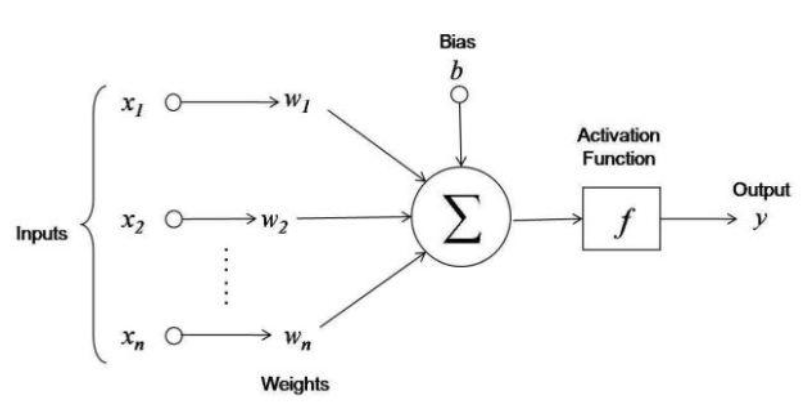
\includegraphics[width=\textwidth]{img/perceptron.png}
	\caption{Perceptron Architecture}
\end{figure}

A \textbf{Perceptron} is a \textit{binary classifier that maps his inputs to a specific output y = f(z), where f() is the \textbf{activation function} of the perceptron.} The inputs are real numbers and the input z of the activation function is obtained as:\\
\begin{equation}
	z = b + \sum_{i = 0}^{N_{L}-1}w_{i}*x_{i}
\end{equation}

Every input $x_{i}$, every weight $w_{i}$ and the bias $b$ are real numbers in the range of $[-1, 1]$. \\
The \textbf{activation function}, in our case, will be a \textbf{sigmoid function}, described as follows:
\begin{figure}[h]
	\centering
	\caption{Sigmoid Function Plot}
	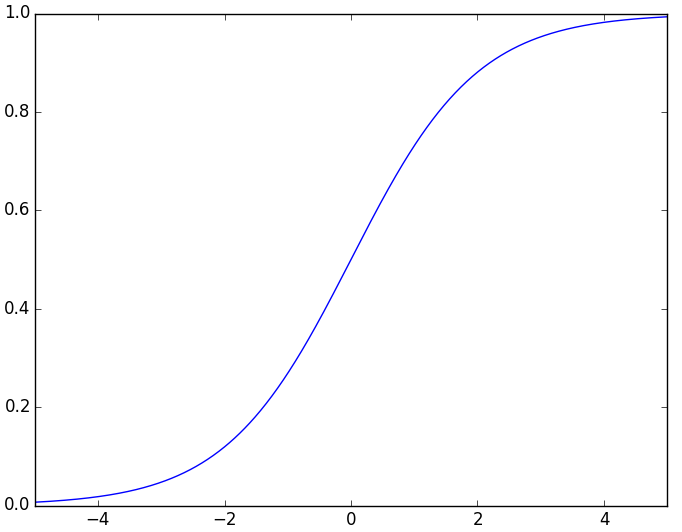
\includegraphics[width=8cm]{img/sigmoid.png}
\end{figure}
\begin{equation}
	y = \dfrac{1}{1+e^{-z}}
\end{equation}
Where $z$ is the result of the equation (1.1).
\section{Applications}

\section{Possible Architectures}
